\documentclass[12pt]{article}
\usepackage{times} 			% use Times New Roman font

\usepackage[margin=1in]{geometry}   % sets 1 inch margins on all sides
\usepackage{hyperref}               % for URL formatting
\usepackage[pdftex]{graphicx}       % So includegraphics will work
\setlength{\parskip}{1em}           % skip 1em between paragraphs
\usepackage{indentfirst}            % indent the first line of each paragraph
\usepackage{datetime}
\usepackage[small, bf]{caption}
\usepackage{listings}               % for code listings
\usepackage{xcolor}                 % for styling code
\usepackage{multirow}
\usepackage{float}
\usepackage{ragged2e}

%New colors defined below
\definecolor{backcolour}{RGB}{246, 246, 246}   % 0xF6, 0xF6, 0xF6
\definecolor{codegreen}{RGB}{16, 124, 2}       % 0x10, 0x7C, 0x02
\definecolor{codepurple}{RGB}{170, 0, 217}     % 0xAA, 0x00, 0xD9
\definecolor{codered}{RGB}{154, 0, 18}         % 0x9A, 0x00, 0x12

%Code listing style named "gcolabstyle" - matches Google Colab
\lstdefinestyle{gcolabstyle}{
  basicstyle=\ttfamily\small,
  backgroundcolor=\color{backcolour},   
  commentstyle=\itshape\color{codegreen},
  keywordstyle=\color{codepurple},
  stringstyle=\color{codered},
  numberstyle=\ttfamily\footnotesize\color{darkgray}, 
  breakatwhitespace=false,         
  breaklines=true,                 
  captionpos=b,                    
  keepspaces=true,                 
  numbers=left,                    
  numbersep=5pt,                  
  showspaces=false,                
  showstringspaces=false,
  showtabs=false,                  
  tabsize=2
}

\lstset{style=gcolabstyle}      %set gcolabstyle code listing

% for fancy page headings
\usepackage{fancyhdr}
\setlength{\headheight}{13.6pt} % to remove fancyhdr warning
\pagestyle{fancy}
\fancyhf{}
\rhead{\small \thepage}
\lhead{\small HW 1, Conner}  % EDIT THIS, REPLACE # with HW number
\chead{\small CS 432, Fall 2020} 

%-------------------------------------------------------------------------
\begin{document}

\begin{centering}
{\large\textbf{HW 1 - Webscience Intro}}\\ % EDIT THIS
                                % REPLACE # with HW num and ADD title
Jacob Conner\\                     % EDIT THIS
September 20, 2020\\                      % EDIT THIS
\end{centering}

%-------------------------------------------------------------------------

% The * after \section just says to not number the sections
\section*{Q1}
Consider the "bow-tie" structure of the web in the Broder et al. paper (http://snap.stanford.edu/class/cs224w-readings/broder00bowtie.pdf) that was described in Week 1.
Now consider the following links (\ref{lst:listNodes}) Draw the resulting graph (either sketch on paper or use another tool) and include an image in your report.)

\begin{lstlisting}[numbers=none, caption=Links, label=lst:listNodes]
A --> B
B --> A
B --> C
C --> D
C --> G
D --> A
D --> H
E --> F
E --> O
F --> G
G --> P
H --> L
J --> N
K --> I
M --> A
N --> L
O --> J
P --> C
\end{lstlisting}

For the above graph, list the nodes (in alphabetical order) that are each of the following categories:
\begin{itemize}
  \item IN:
  \item SCC:
  \item OUT:
  \item Tendrils:
	\begin{itemize}
		\item indicate if the tendril is reachable from IN or can reach OUT
	\end{itemize}
\item Tubes:
	\begin{itemize}
		\item explain how the nodes serve as tubes
	\end{itemize}
\item Disconnected:
\end{itemize}

\subsection*{Answer}

\emph{All figures must have a caption and must be referenced in the text. Example below.}

Figure \ref{fig:bowTieGraph} was created using the \textit{Dia} diagramming tool \cite{dia} and shows the relationships between each node.

\begin{figure}[h]
    \centering
    % trim and clip are used to crop the image, trim=left bottom right top
    % width sets max width, height will be scaled appropriately
    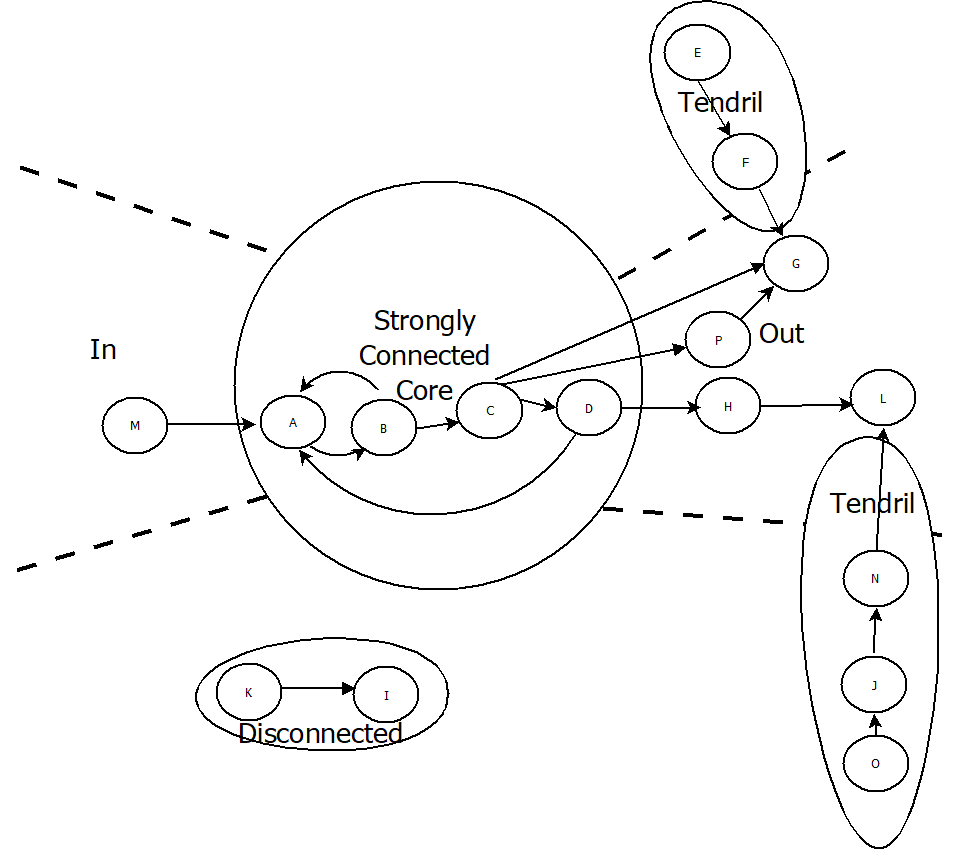
\includegraphics[trim=10 10 10 50, clip, width=\textwidth] {Q1/Q1.png}
    \caption{Bow-Tie Graph representing relationship between nodes}
    \label{fig:bowTieGraph}
\end{figure}

\begin{itemize}
  \item IN: M
  \item SCC: A, B, C, D
  \item OUT: G, H, L,
  \item Tendrils : NONE
	\begin{itemize}
		\item Reaching outward (FROM IN): NONE
		\item: Reaching in (to OUT): E, F, J, N, O
	\end{itemize}
\item Tubes: NONE
\item Disconnected: K, I
\end{itemize}

\subsection*{Discussion}
The very first step to identify types of nodes is to identify what portions of the graph are strongly condnected. The graph is "strongly connected if there is path beween all pairs of vertices" \cite{GeeksForGeeks}. In this graph there are four strongly connected nodes, A, B, C, and D. \ref{1} lists the strongly connected component nodes (SCC) and the paths beween each of these nodes. Since these four nodes are all strongly connected, they form the Strongly Connected Component in the graph. The OUT nodes are the nodes that only link out from a strongly connected component node or another OUT node. In this case, the OUT nodes consist of nodes G  and P which links out from the SCC node C, node H that links from the SCC node D, and node L that links from the OUT node H. Similarly, the IN nodes were identified as the nodes that only link in to another IN node or a SCC node. In this graph there is only one IN node, M, which links in to to the SCC node A. Tendrils are the groups of nodes that either link out from an IN node or link in to an OUT node. In this graph, there were not any nodes linking outward from the one IN node, but there were three nodes, J, N, and O, that reached in to the OUT node L. Tubes are the nodes that that link between IN and OUT nodes without going through the SCC. Since there were no nodes linking from IN to the OUT nodes, there were no tubes. Then disconnected nodes were the nodes that do not connect to a  SCC, IN, or OUT noded. In this graph, there were two disconnected nodes, K and I.. Node K can connect to Node I but cannot connect to anything else and Node I serves only as a destination for Node K and does not link to anything else. 

Since this graph is a miniature representation of the web, the most interesting observation we can glean from the graph is that there are several factors that will prevent search engines and web crawlers from identifying every website simply by following links. The first limiation to indexing the whole web is that some nodes are disconnected and are not linked to from any other website. Since no websites link to these disconnected ndoes, it is simply not possible to uncover these websites. A second limitation is depending on where you are in the graph, will determine how much of the remainder of the web can be uncovered. If a webcrawler started indexing at the SCC node A, it would be able to find most of the nodes in this graph, but I would never be able to reach node M since it is merely linking to A and A does not link back to M. A webcrawler would also never be able to uncover any of the tendrils since they link to OUT nodes, but the OUT nodes do not link back to them. If by some chance a webcrawler started on an OUT node then the number of websites that could be indexed would be relatively small as only OUT nodes could be indexed at that point. Clearly, through this graph, we are able to see some of the limitations of webcrawlers that follow links from one page to another

\begin{table}[h]
\centering
\caption{SCC Links}
\label{tbl:scclinks}
\begin{tabular}{|l|l|l|l|l|}
\hline
\textbf{ } & \textbf{A} & \textbf{B} & \textbf{C} & \textbf{D} \\ \hline
A & X & A,B & A,B,C & A,B,C,D \\ \hline
B & B,A & X & B,C & B,C,D \\ \hline
C & C,D,A & C,D,A,B & X & C,D \\ \hline
D & D,A & D,A,B & D,A,B,C & X \\ \hline
\end{tabular}
\end{table}

\section*{Q2}
Demonstrate that you know how to use curl and are familiar with the available options.



a) In a single curl command, request the URI, show the HTTP response headers, follow any redirects, and change the User-Agent HTTP request field to "CS432/532". Show command you used and the result of your execution on the command line. (Either take a screenshot of your terminal or copy/paste into a code segment.)

b) Then make the same request again, but without showing the HTTP response headers and with saving the HTML output to a file. Show the command you used and the result of your execution on the command line. View that file in a browser and take a screenshot.

c) Finally, load the URI directly from your browser and take a screenshot.

Explain the results you get for each of these steps.
\subsection*{Answer}
\subsubsection*{a)}
\begin{lstlisting}[numbers=none, caption=Command, label=lst:q2ACommand]
curl -i -L -A "CS432/532" http://www.cs.odu.edu/~mweigle/courses/cs532/ua_echo.php
\end{lstlisting}
\begin{lstlisting}[numbers=none,
		        caption={curl command to get the GET response and header, redirects and send a User-Agent header propety}, 
			label=lst:q2AResponse]
  % Total    % Received % Xferd  Average Speed   Time    Time     Time  Current
                                 Dload  Upload   Total   Spent    Left  Speed
100   178  100   178    0     0   2282      0 --:--:-- --:--:-- --:--:--  2825
100   114  100   114    0     0    561      0 --:--:-- --:--:-- --:--:--  1461HTTP/1.1 301 Moved Permanently
Server: nginx
Date: Sat, 29 Aug 2020 15:08:24 GMT
Content-Type: text/html
Content-Length: 178
Connection: keep-alive
Location: https://www.cs.odu.edu/~mweigle/courses/cs532/ua_echo.php

HTTP/1.1 200 OK
Server: nginx
Date: Sat, 29 Aug 2020 15:08:24 GMT
Content-Type: text/html; charset=UTF-8
Content-Length: 114
Connection: keep-alive
Vary: Accept-Encoding
X-Powered-By: PHP/5.6.40

<!DOCTYPE html>
<html>
<body>

<br/>USER AGENT ECHO
<br/><br/>
<b>User-Agent:</b> CS432/532<br/>

</body>
</html>
\end{lstlisting}

The curl command is used to make HTTP GET Requests. the -i  or --include flag is used to specify curl to include the headers and the response. The -L or --location flag is used to request the header 
and response for all redirects. The -A or --user-agent flag specifies the User-Agent property in the header that is sends to the string next to it. IN this case the User-Agent sent is "CS432/5432".
Then the last part of the curl command is the URI(s) for the webserver(s) that we are making a HTTP GET request to \cite{curlManPage}.

\subsubsection*{b)}
\begin{lstlisting}[numbers=none, caption="curl command to get headers only for all redirects and sets the User-Agent header property", label=lst:q2BCommand]
curl -o response.html -L -A "CS432/532" http://www.cs.odu.edu/\~mweigle/courses/cs532/ua\_echo.php
\end{lstlisting}

\lstinputlisting[language=HTML, caption=response.html, label=lst:responseHtml]{Q2/response.html}
\begin{figure}[h]
    \centering
    % trim and clip are used to crop the image, trim=left bottom right top
    % width sets max width, height will be scaled appropriately
    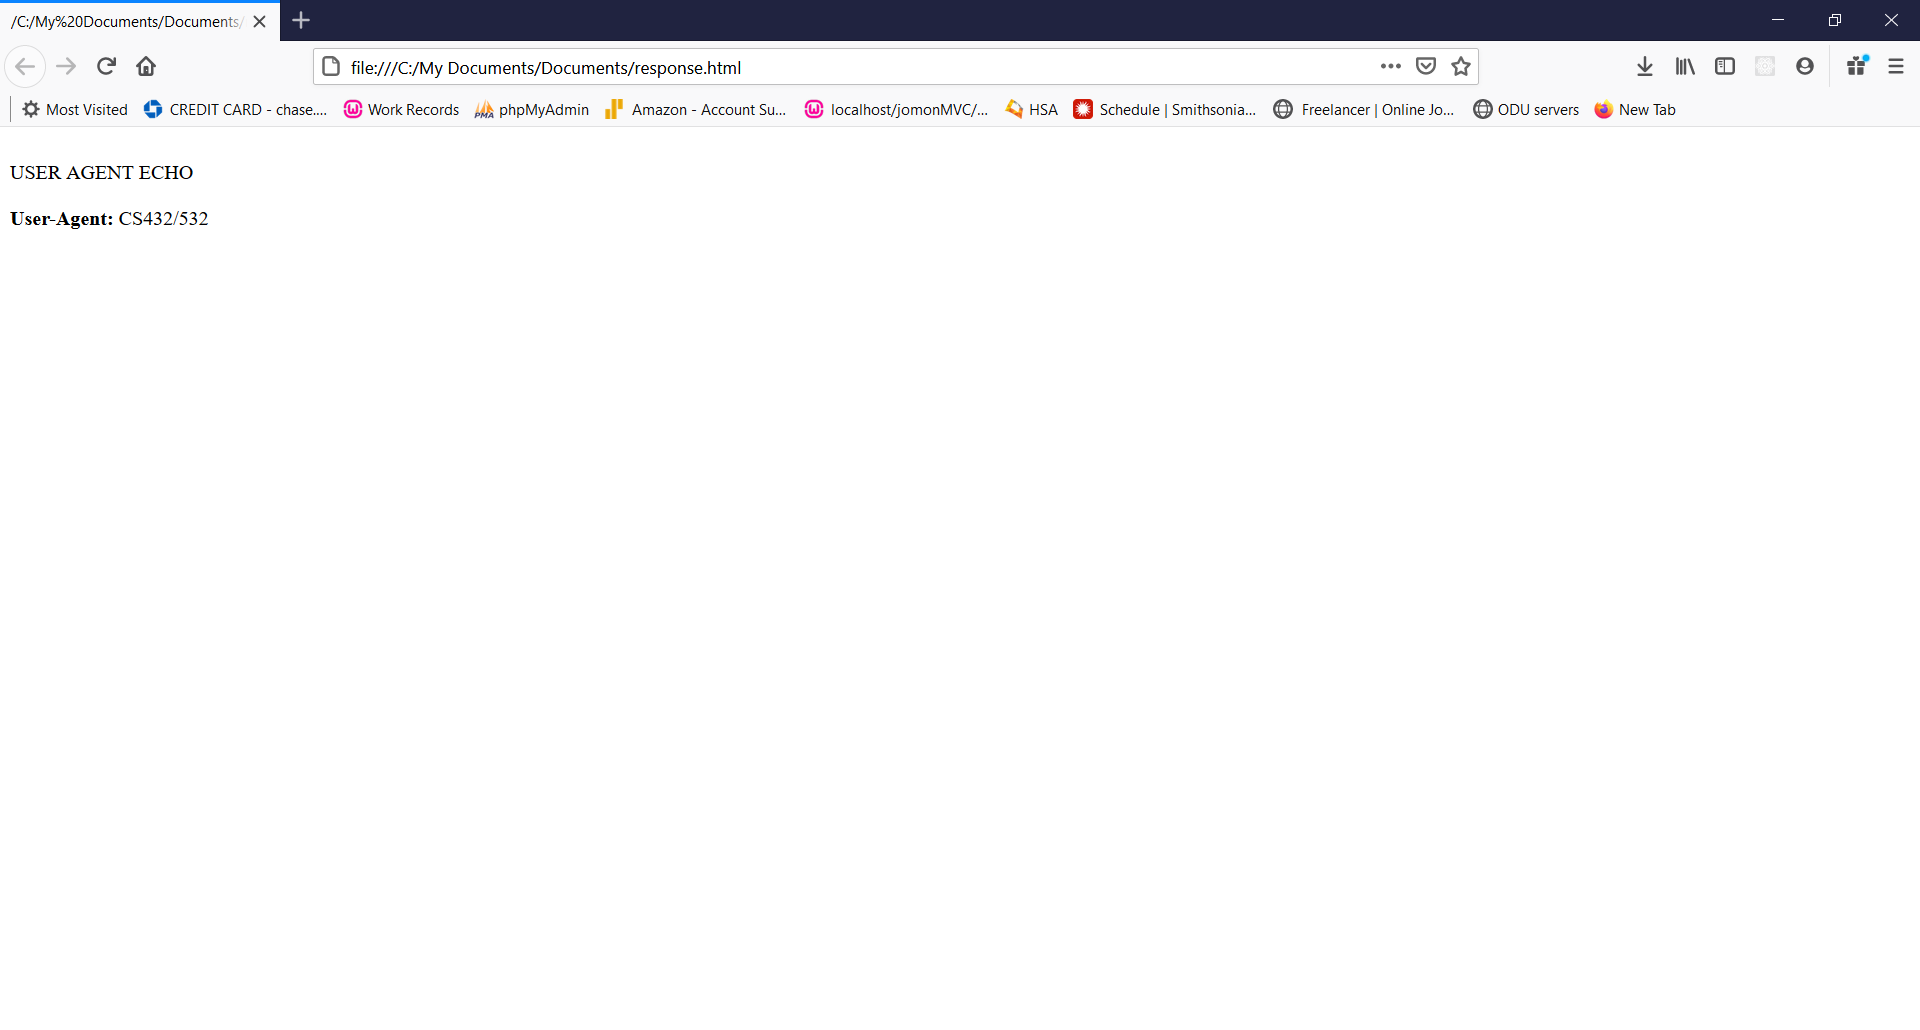
\includegraphics[trim=0 400 300 50, clip, width=\textwidth] {Q2/Q2b_Screenshot.png}
    \caption{Browser representation of the GET request response.html}
    \label{fig:q2BResponse}
\end{figure}

This command is similar to the previous command in part a. However since we do not need the header information,, so the -i --include flag has been omitted. I have also added the -o output flag to copy the resulting
response from the server into the file response.html. \ref{lst:responseHtml} shows this output from the GET request. The response.html file is a fairly simple html file with a body tag enclosing one set of bold tags surrounding the words User-Agent, and  the value of our User-Agent property (CS432/532) in the GET request header. The browser representation of the response is displayed in \ref{fig:q2BResponse}.


\subsubsection*{c)}
\begin{figure}[h]
    \centering
    % trim and clip are used to crop the image, trim=left bottom right top
    % width sets max width, height will be scaled appropriately
    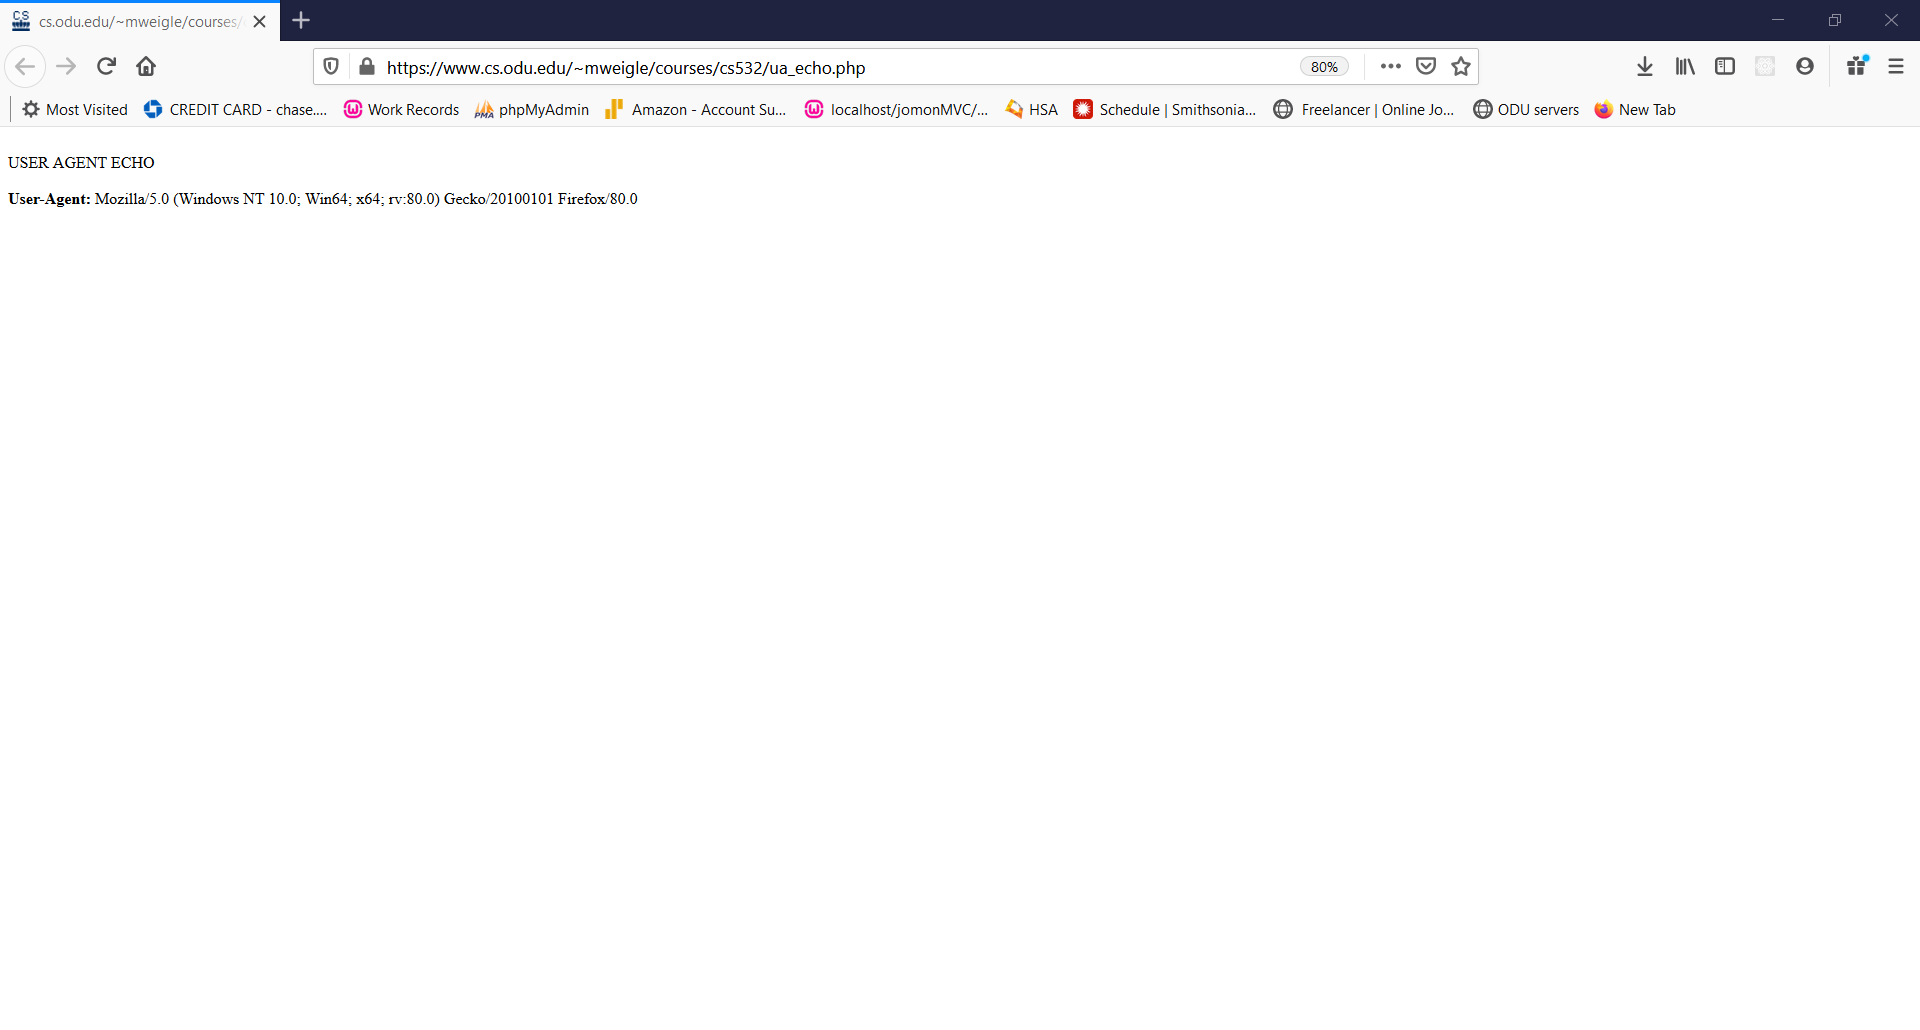
\includegraphics[trim=0 400 300 50, clip, width=\textwidth] {Q2/Q2c_Screenshot.png}
    \caption{Browser representation of GET request to https://www.cs.odu.edu/~mweigle/courses/cs532/ua\_echo.php }
    \label{fig:q2CResponse}
\end{figure}

If a browser navigates to https://www.cs.odu.edu/\~mweigle/courses/cs532/ua\_echo.php, the browser sends the GET HTTP request in the background and receives the Response and creates a representation of
 the response which will look similar to \ref{fig:q2CResponse}. It looks very similar to the previous response.html retrieved from the curl command, but in the browser the User-Agent shows a different string. On
the computer I am currently using, I am running Windows 10 64-bit and running Firefox, so the browser uses that information to send a string to the "User-Agent" property in the header of the GET request to help the webserver identify
how I am accessing this page. If I were to use a different browser such as Chrome or if I ran Firefox on a linux distribution, I would get a different string. On every GET Request submitted by the browser, this same
User-Agent string is submitted.

\subsection*{Discussion}
In this section, different methods of create HTTP GET Requests was examined. In the first two questions, the GET Request was created using the curl command and the headers had to be specified in the command line. In this case only one property was sent in the header and that was "User-Agent".  Then in the last question, a browser was used to issue a GET request for https://www.cs.odu.edu/~mweigle/courses/cs532/ua\_echo.php and the browser automatically created a User-Agent string for the header. One interesting observation from this exercise is that a webserver can very easily identify if a GET request is coming from a browser or another application because a browser sends a header with a unique "User-Agent" string by default and other methods may not. 
\section*{Q3}
Write a Python program to find links to PDFs in a webpage.

Your program must do the following:
\begin{itemize}
    \item take the URI of a webpage as a command-line argument
    \item extract all the links from the page
    \item for each link, use the Content-Type HTTP response header to determine if the link references a PDF file
    \item for all links that reference a PDF file, print the original URI (found in the source of the original HTML), the final URI (after any redirects), and the number of bytes in the PDF file. (Hint: Content-Length HTTP response header)
\end{itemize}
Show that the program works on 3 different URIs, one of which must be https://www.cs.odu.edu/~mweigle/courses/cs532/pdfs.html
Here is a snippet of the expected operation:

\begin{lstlisting}[numbers=none, caption=Expected Output, label=lst:q3ExpectedOutput]
% python3 findPDFs.py https://www.cs.odu.edu/~mweigle/courses/cs532/pdfs.html

URI: http://www.cs.odu.edu/~mln/pubs/ht-2015/hypertext-2015-temporal-violations.pdf
Final URI: https://www.cs.odu.edu/~mln/pubs/ht-2015/hypertext-2015-temporal-violations.pdf
Content Length: 2,184,076 bytes

URI: http://www.cs.odu.edu/~mln/pubs/tpdl-2015/tpdl-2015-annotations.pdf
Final URI: https://www.cs.odu.edu/~mln/pubs/tpdl-2015/tpdl-2015-annotations.pdf
Content Length: 622,981 bytes
\end{lstlisting}

\subsection*{Answer}
Listing \ref{lst:findPDFs} is the imported code I used to scrape pdf files from webpages.
\subsubsection*{Program Code}
\lstinputlisting[language=Python, caption=findPDFs.py, label=lst:findPDFs]{Q3/findPDFs.py}

Below I have provided screenshots of various sample output from the findPDFs.py scraper. 
\subsection*{Test 0: Dr. Weigle's PDFs} 

\ref{fig:q3ResponseWeigle} is the output I received after running the findPDFs.py scraper on https://www.cs.odu.edu/\~ mweigle/courses/cs532/pdfs.html 
\begin{figure}[H]
    \centering
    % trim and clip are used to crop the image, trim=left bottom right top
    % width sets max width, height will be scaled appropriately
    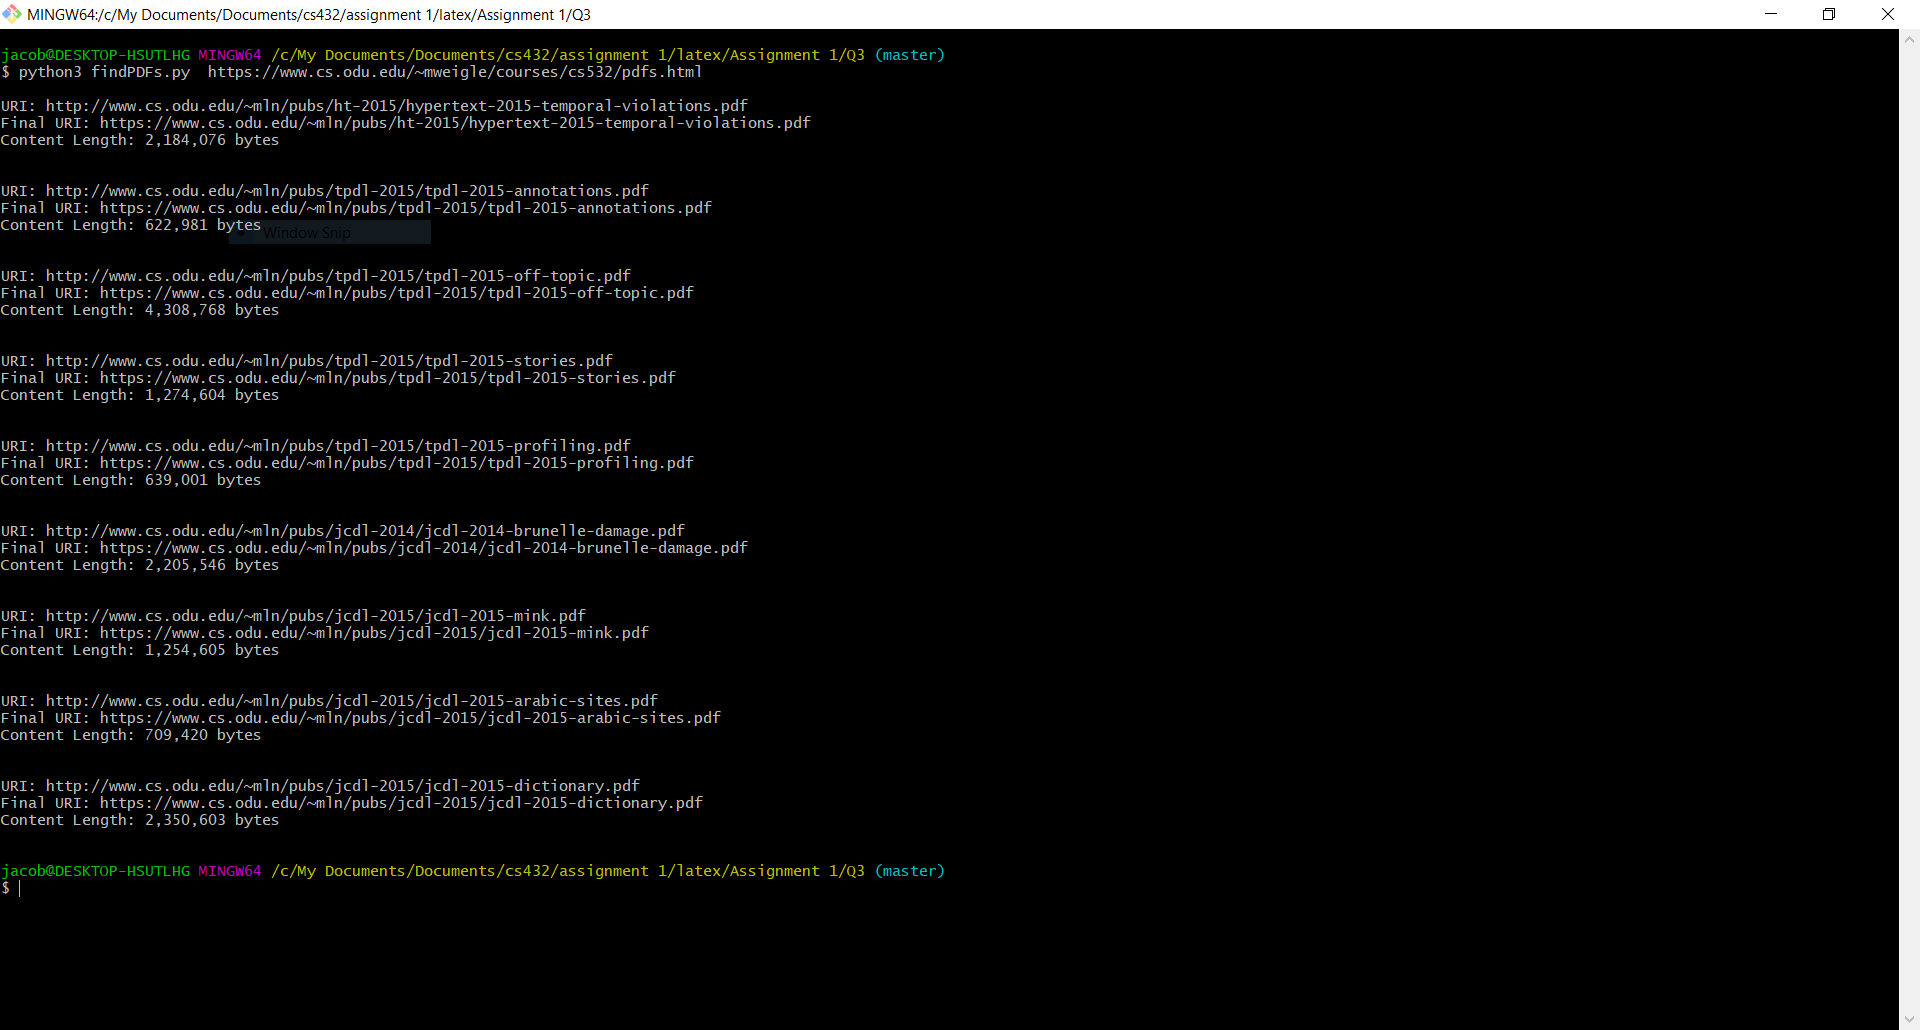
\includegraphics[trim=0 50 400 20, clip, width=\textwidth] {Q3/q3_weiglePdfs.png}
    \caption{findPDFs.py results for https://www.cs.odu.edu/\~ mwei-
gle/courses/cs532/pdfs.html}
    \label{fig:q3ResponseWeigle}
\end{figure}

\subsection*{Test 1: Ubuntu Documentation} 
\ref{fig:q3ResponseUbuntu} is the output I received after running the findPDFs.py scraper on the Ubuntu manual page (https://help.ubuntu.com/)
\begin{figure}[H]
    \centering
    % trim and clip are used to crop the image, trim=left bottom right top
    % width sets max width, height will be scaled appropriately
    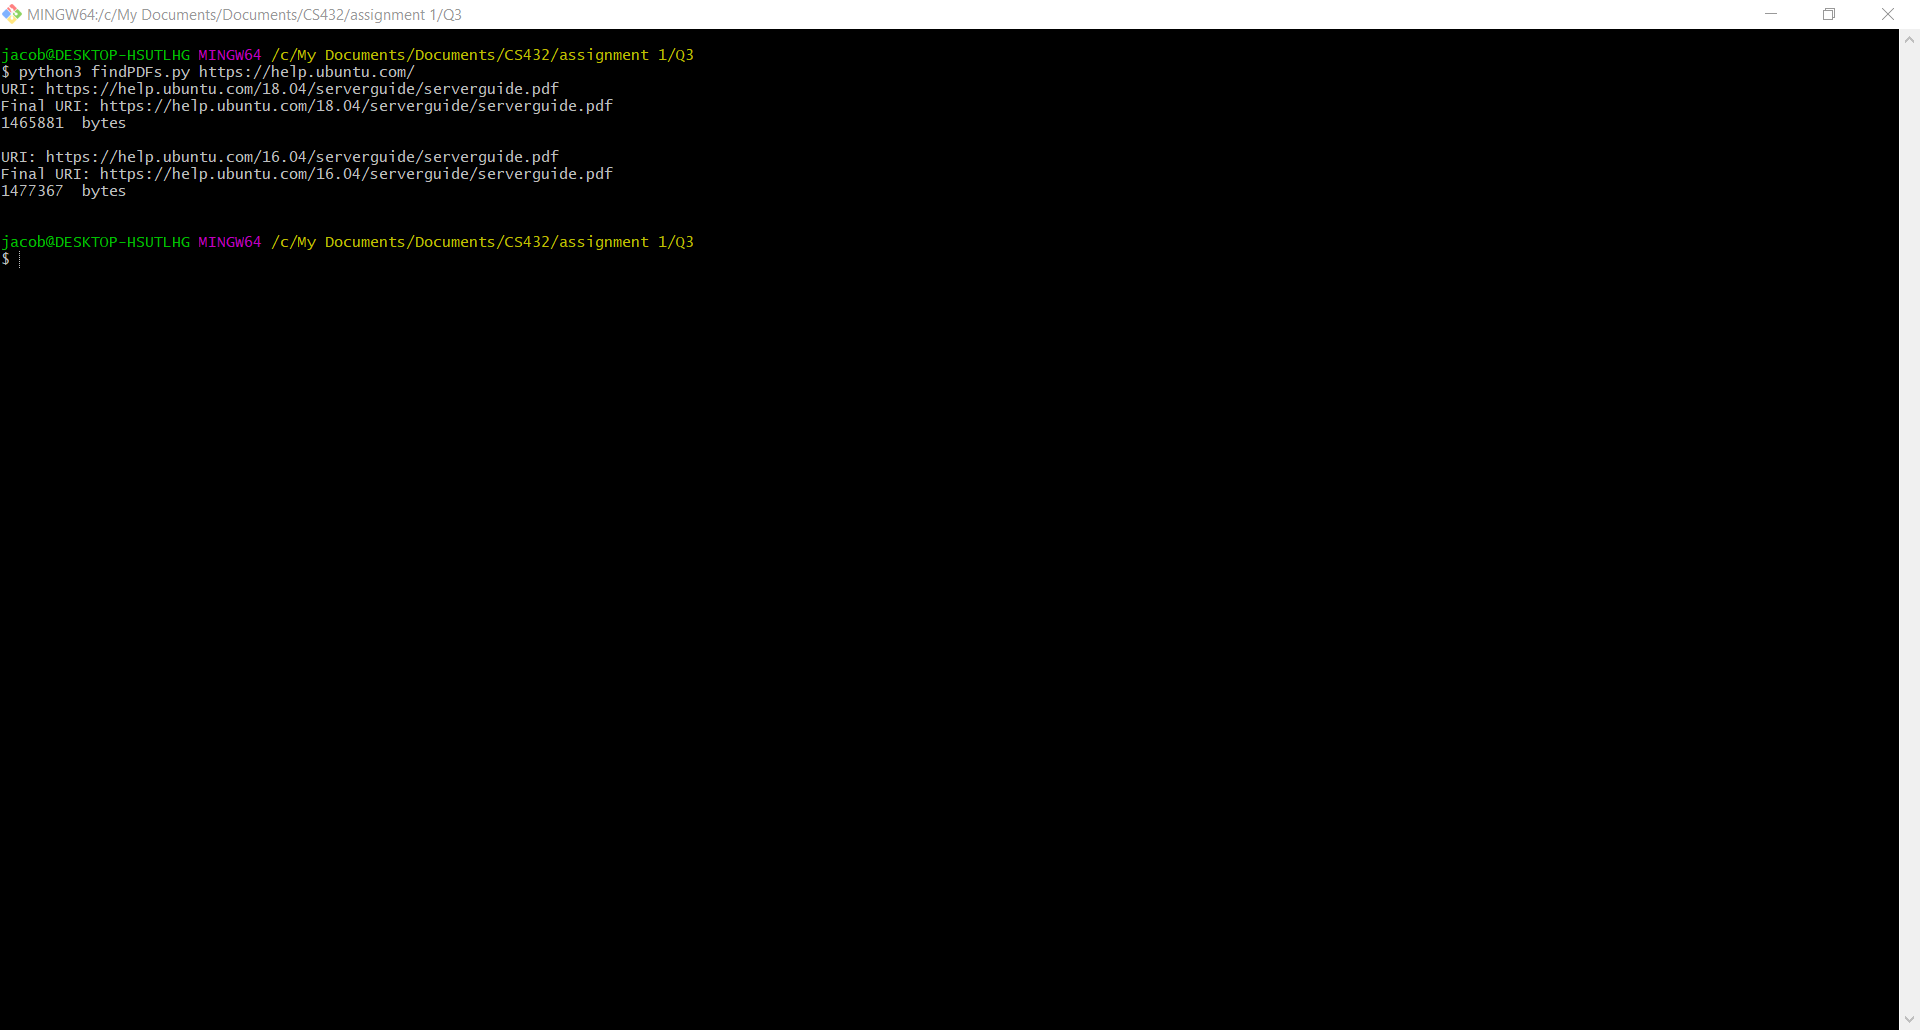
\includegraphics[trim=0 20 400 20, clip, width=\textwidth] {Q3/q3_ubuntuHelp.png}
    \caption{findPDFs.py results for https://help.ubuntu.com/}
    \label{fig:q3ResponseUbuntu}
\end{figure}

\subsection*{Test 2: CRAN-R R Documentation} 
\ref{fig:q3ResponsecranR_1} and \ref{fig:q3ResponsecranR_2} are screenshots of the output I received after running the findPDFs.py scraper on the CRAN-R R programming manuals page (https://cran.r-project.org/manuals.html)
\begin{figure}[H]
    \centering
    % trim and clip are used to crop the image, trim=left bottom right top
    % width sets max width, height will be scaled appropriately
    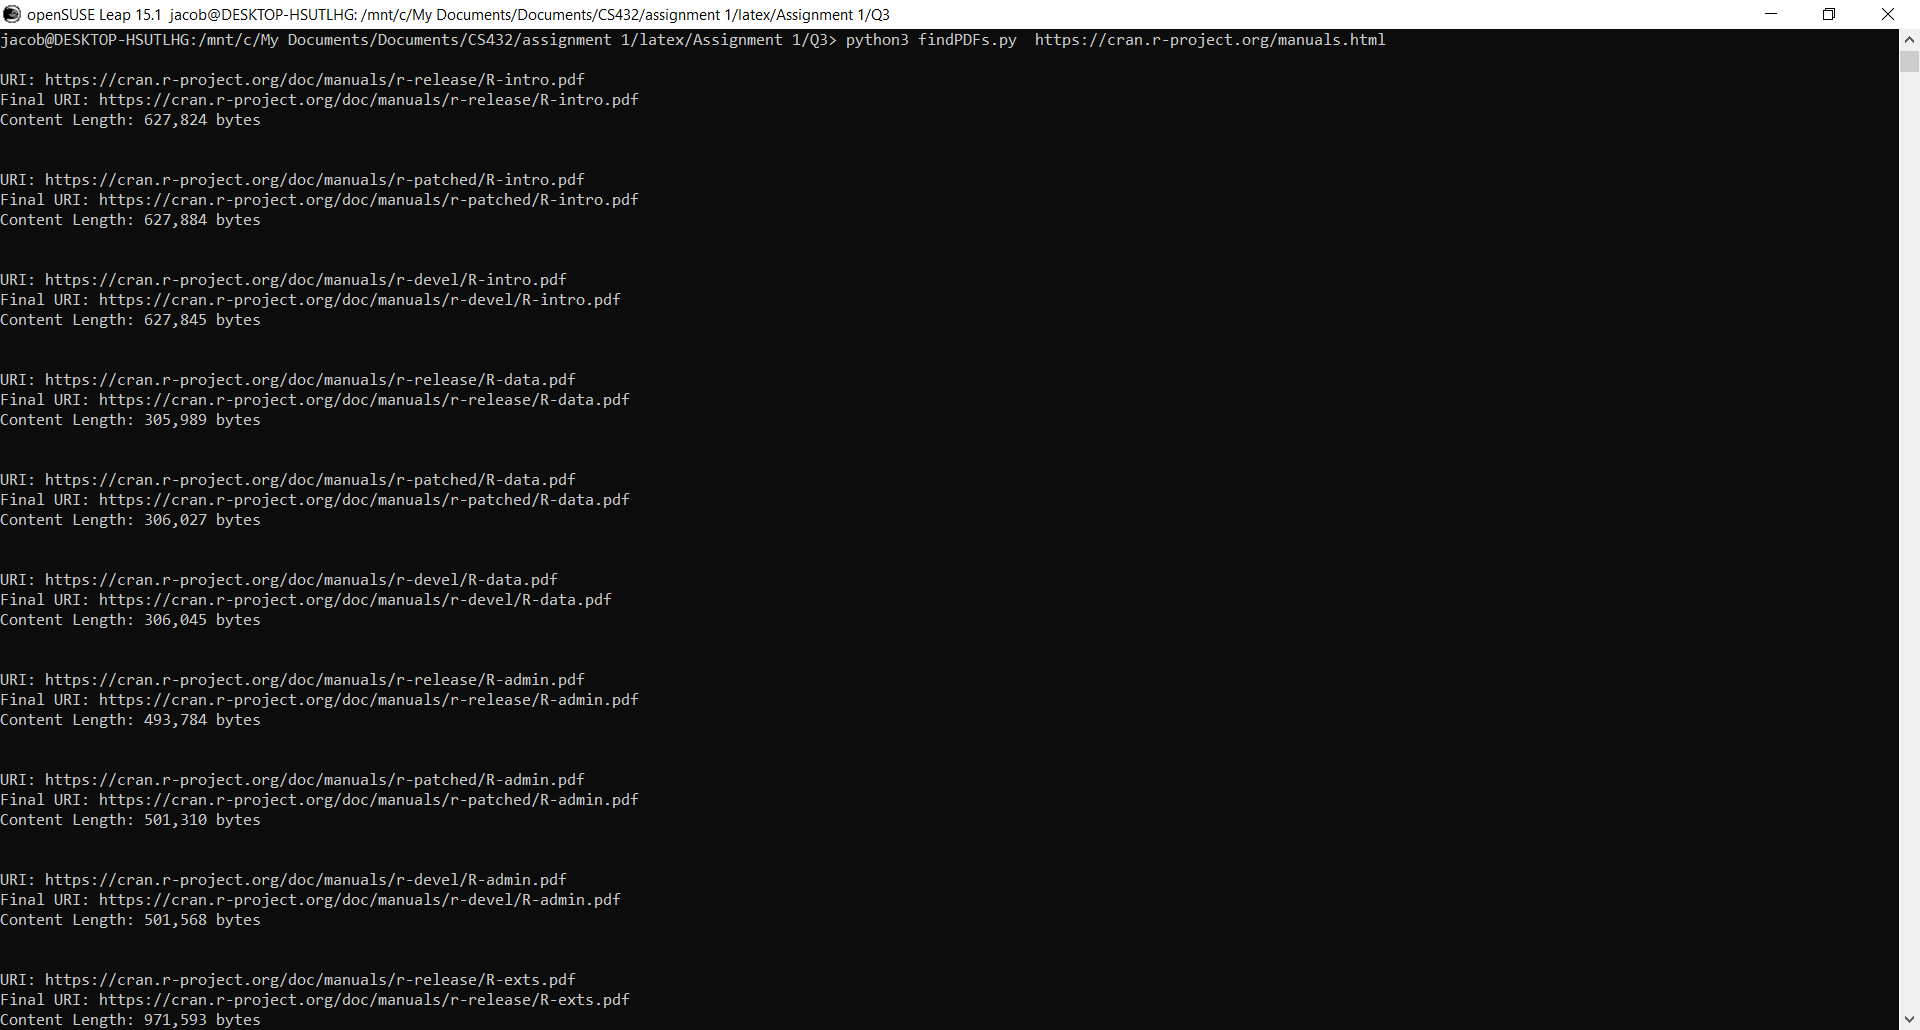
\includegraphics[trim=0 0 400 20, clip, width=\textwidth] {Q3/q3_cranRManuals.png}
    \caption{findPDFs.py results for https://cran.r-project.org/manuals.html}
    \label{fig:q3ResponsecranR_1}
\end{figure}

\begin{figure}[H]
    \centering
    % trim and clip are used to crop the image, trim=left bottom right top
    % width sets max width, height will be scaled appropriately
    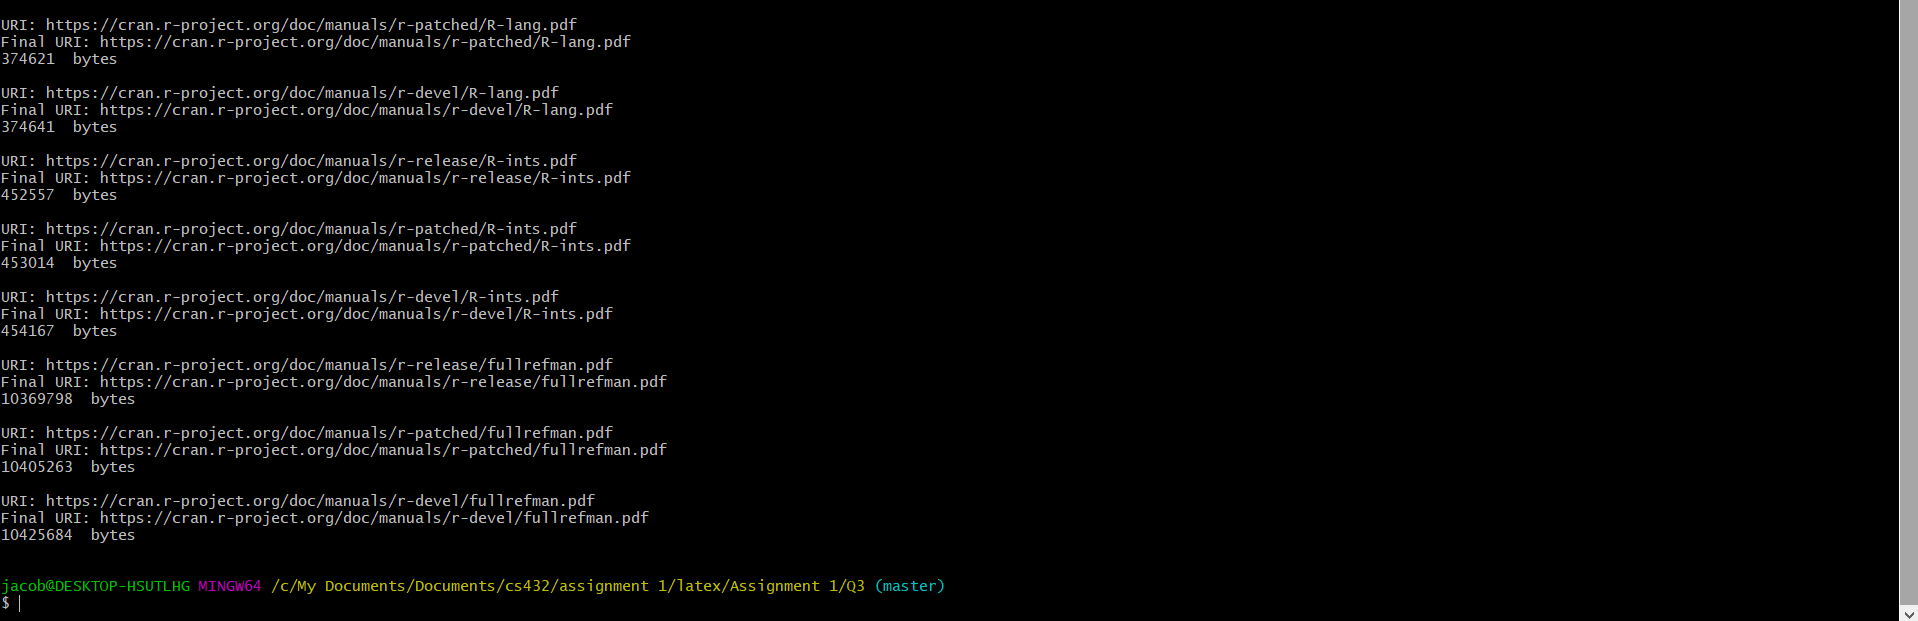
\includegraphics[trim=0 30 400 10, clip, width=\textwidth] {Q3/q3_cranRManuals2.png}
    \caption{findPDFs.py results for https://cran.r-project.org/manuals.html}
    \label{fig:q3ResponsecranR_2}
\end{figure}

\subsection*{Test 3: Society for East Asian Archaeology} 
\ref{fig:q3ResponseSEAA_1} is a screenshot of the output I received after running the findPDFs.py scraper on the Society of East Asian Archaeology's 2016 bulletin page (https://seaa-web.org/publications/bseaa/bulletin-society-east-asian-archaeology)
\begin{figure}[H]
    \centering
    % trim and clip are used to crop the image, trim=left bottom right top
    % width sets max width, height will be scaled appropriately
    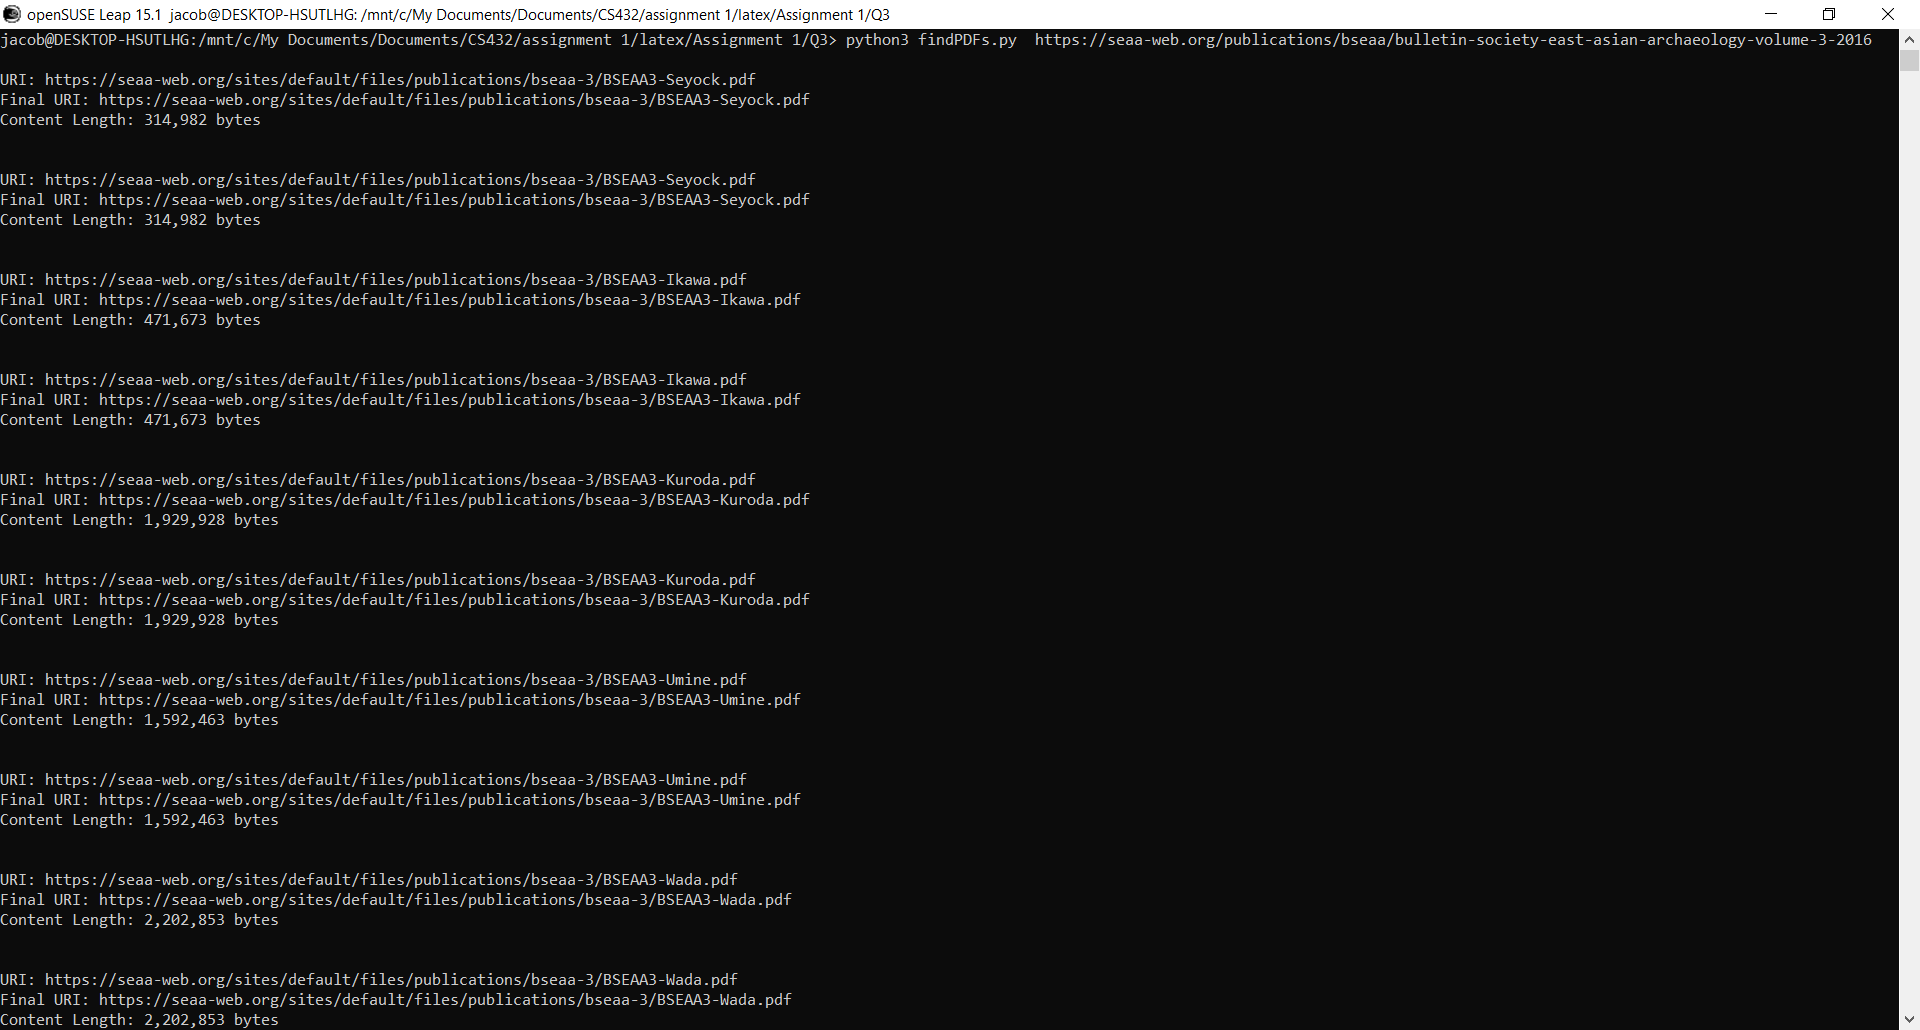
\includegraphics[trim=0 20 400 20, clip, width=\textwidth] {Q3/q3-seaaBulletin2016.png}
    \caption{findPDFs.py results for https://seaa-web.org/publications/bseaa/bulletin-society-east-asian-archaeology}
    \label{fig:q3ResponseSEAA_1}
\end{figure}


\subsection*{Discussion}

The Python code above generates a console program that accepts a url as a command-line argument from the user. If no url is provided, the program exits. A HTTP GET request is made to the URL along with a header with the "User-Agent" property to allow the code to run on more webservers that may reject GET requests that omit this property. Once a response is received from the webserver is received, the resulting text from the response is parsed using the BeautifulSoup library to retrieve all of the anchor ('a') tags in the document. Then every anchor's 'href' attribute is tested to see if it is an absolute path. If the url is a relative path, i tis converted to an absolute path. After the link is in the correct form, it is checked to see if it is a pdf and another GET Request is made for each URL. The resulting response from the GET request is used to print the URI, Final URI and file size output to the console. 

In order to accomplish task, I have created a main function with 6 other functions. The main function begins with retrieving the url  from the user input. The user input is handled using the checkForArguments function and it makes use of the sys library's argv function to get the first command from the user. A conditional is used to check if the the argv variable exists and if not, it exits the program. This function only checks to make sure the url argument is provided and does not evaluate if it is a valid url or not.

The user provided URL is then validated with the The validateRequest function. Since some webservers do not like webscrapers and will reject their GET requests, the validateRequest function begins with building a header and generates a "User-Agent" string to mimic a browser's "User-Agent" string using a modified version of the GET\_UA function.\cite{randomizeUserAgent}. TheThe GET\_UA function is simply a list of "User-Agent" strings that I created using Firefox, Chrome, Edge, Opera, and Internet Explore n Windows 10. These User-Agent strings were obtained by visiting whatismyip.com \cite{whatIsMyIp} but technically, I could have obtained them from the website used in Question 2 as well. The GET\_UA  function use Python's built in random library to pick one of these "User-Agent" strings at random. The validateRequest function uses the resulting "User-Agent" string to build a header. A try catch block is used to try a HTTP GET request using the requests library. If a response is received, the validateRequest function returns the response and if it fails, an Exception is generated and the function returns None. 

After retrieving the response, the main function uses the BeautifulSoup library to parse the HTML to retrieve all anchor tags. There are numerous HTML parsers available including Python's built in HTMLParser library, but in order to make use of that library, a subclass of HTMLParser has to be created and we must override various methods to get the anchor tags. The BeautifulSoup library is able to do this with a single line that initializes the BeautifulSoup object with theGET request's response text and then calls the FindAll method to retrieve all anchor tags. Due tothis simplicity, BeautifulSoup was used.  BeautifulSoup returns a list-like object that is iterated through using a for loop in order to check each anchor tag's 'href' attribute. 

Now that I have a list of links, I need to format them so they are ready for the response requests. First, I verify that the url is an absolute path, because many websites like to use relative paths to make the code easier to port between testing and production environments. I have modified an absolutePath function \cite{stackOverflowRelativePath} to check if a url starts with "http://www" or "https://www" and if not, the function assumes the link found was a relative url. The urljoin method is used from the UrlLib library to convert the relative url to an absolute url.

Next, next the checkIfPDFRegEx function is used to check if the link is a pdf. This function uses regular expressions with the re libary to check if a url ends in '.pdf' and if it ends in .pdf, the function assumes the link is a pdf. This will find all pdfs as long as the file has the extension. An alternative approach to checking for PDFs is to make a GET or HEAD request using the requests library to read the "Content-Type" property from the header.  If the property exists, you can check if it is is "application/pdf" and if so, the response must be a pdf. Unfortunately, the "Content-Type" property does not always exist in every header and it requires a lot of extra GET or HEAD requests that could lead to a webserver blocking all requests from the webscraper. Since thiis approaach does not always work, I abandoned the Header approach for PDF identification for the regular expression approach. After verifying the url is a pdf link, the checkIfPDFRegEx function calls the validateRequest function to generate a new GET request and returns the response. If a link is not a PDF, then the function returns None. 

I added one more check in the main function to make sure a pdf link is valid by retrieving the response from the GET request and verifying the final URI in the header ends in a .pdf by running the checkIfPDFRegEx function on the response's url property. If the final URI is not a link ending in .pdf, then the link is likely mistyped on the website or links to a location that no longer exists. I ran into this issue while visiting the Society for East Asian Archaeology's site \cite{bulletin2016SEAA}.  \ref{fig:q3SEAA_badHTML}, shows three links that appaer to be applied at the end of the link to the article by Wada on this page. I examined these links using curl and received output sunukar to \ref{fig:q3SEAA_badHTML_curl}, which reveals these links ending in .pdf are ultimately linking back to the page that contained those links, which is common on some webservers when typos occur on links. HTML typos like this occur all of the time, so this additional step to validate the final URI from the response was included in this program.

\begin{figure}[H]
    \centering
    % trim and clip are used to crop the image, trim=left bottom right top
    % width sets max width, height will be scaled appropriately
    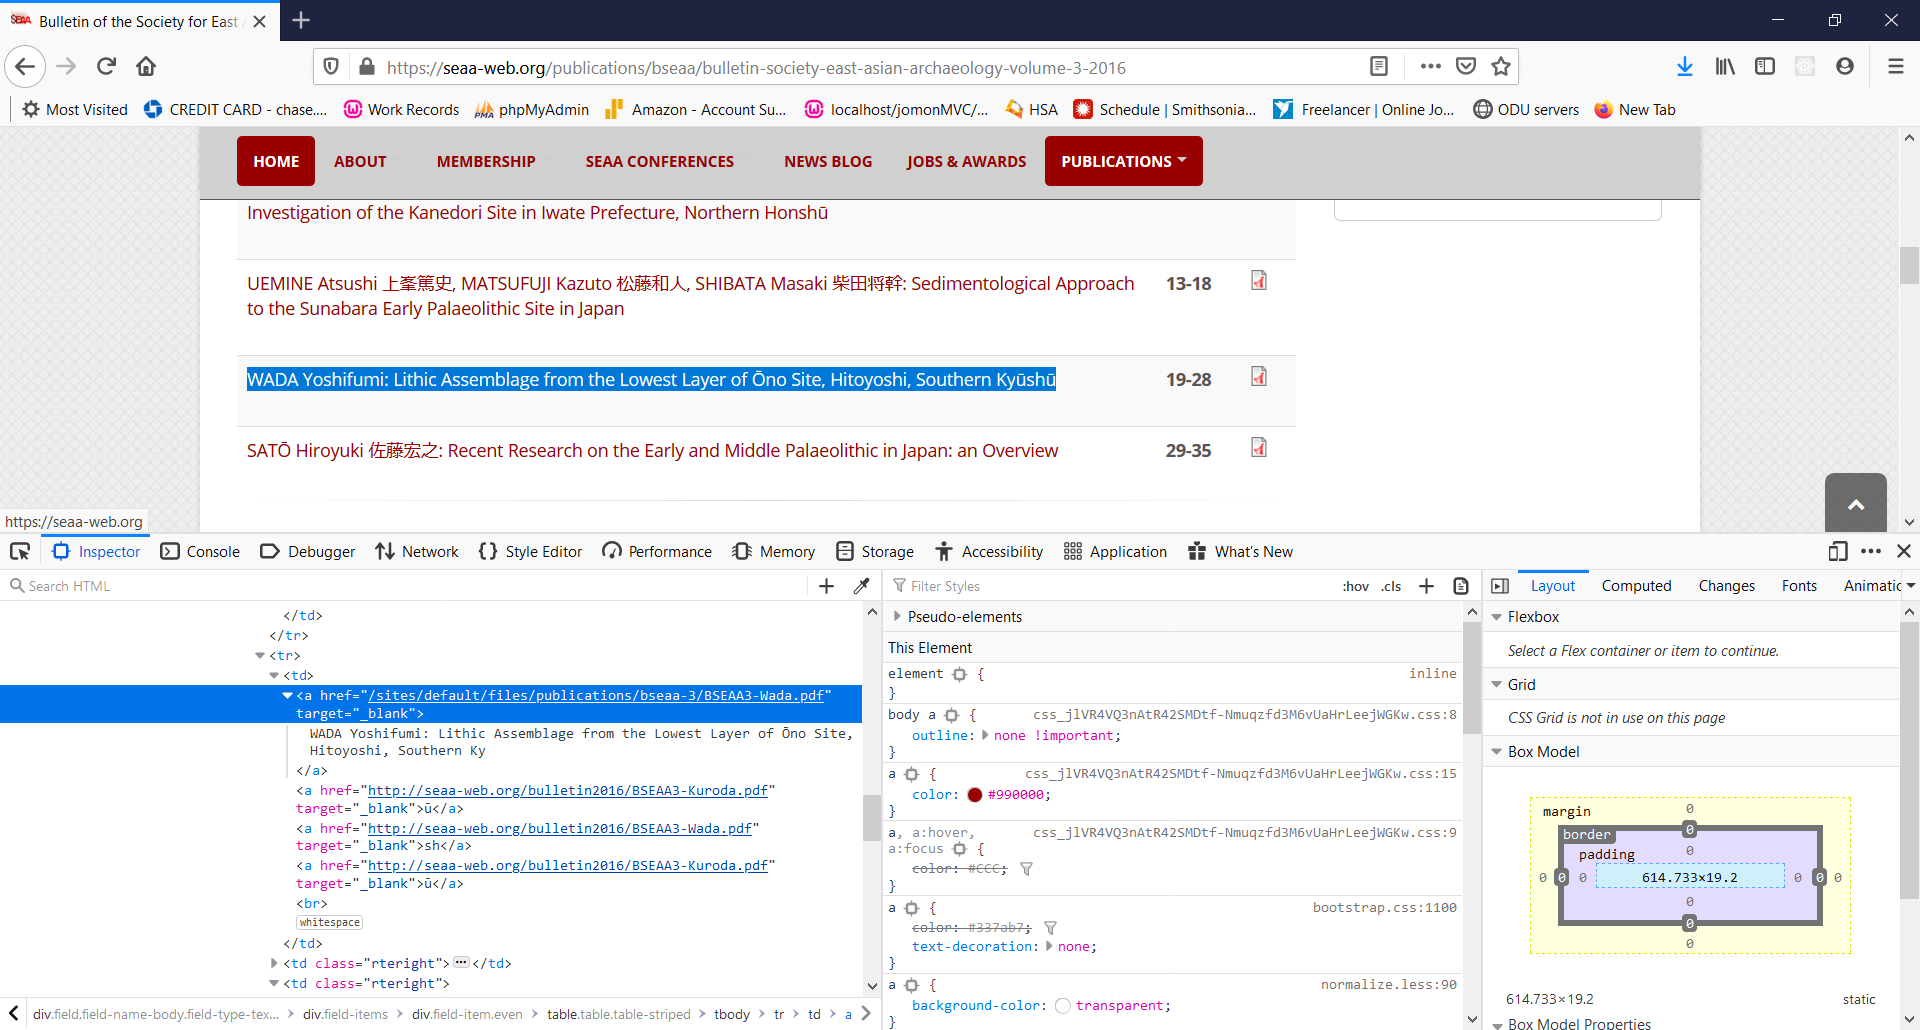
\includegraphics[trim=0 60 10 20, clip, width=\textwidth] {Q3/seaaBadHTML.png}
    \caption{Html Errors on SEAA website with incorrect pdf links. }
    \label{fig:q3SEAA_badHTML}
\end{figure}

\begin{figure}[H]
    \centering
    % trim and clip are used to crop the image, trim=left bottom right top
    % width sets max width, height will be scaled appropriately
    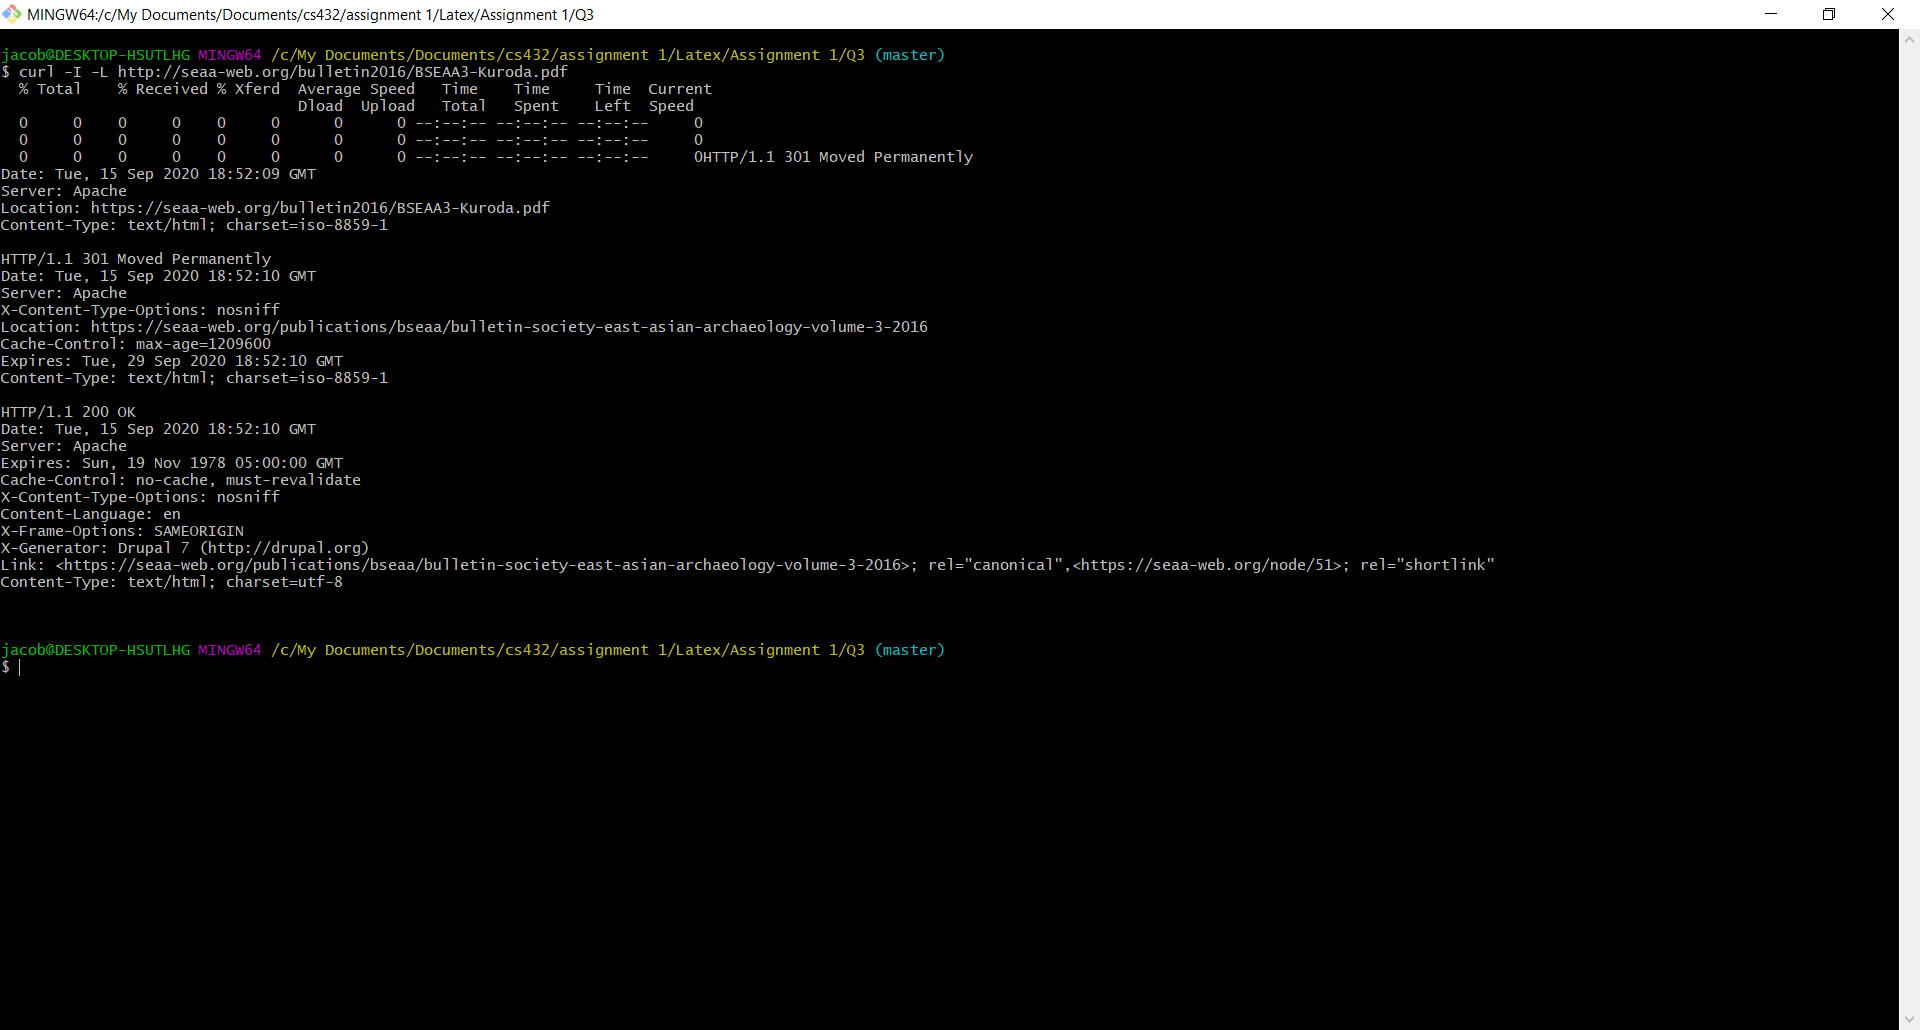
\includegraphics[trim=0 60 10 20, clip, width=\textwidth] {Q3/seaaBadHTML_curl.png}
    \caption{Html Errors on SEAA website with incorrect pdf links. }
    \label{fig:q3SEAA_badHTML_curl}
\end{figure}


The main function ends by calling a the printResult function on all of the responses returned from checkIfPDFRegEx. This function displays the original URI, the final URI (after any redirects) and the size of the pdf file. The URI is created using the original link url (after converting to an absolute path). The final URI is obtained using the GET request response's url property. The requests library by default will set the url to the final redirect unless the GET request is sent with an additional argument of "allow-redirects=False". If allow-redirects is set to false, then GET requests would have to be made on the resulting response.url until the response."status\_code" is no longer 300, 301, 302, 303, 307, or 308. This is quite inefficient and lots of GET requests to a server in a short period of time, increases the likleihood of the server blocking the webscraper. Instead, a normal GET request using the requests library can be used and the url property of the response is the final URI after any redirects. If a history of redirects is needed, the history property of the response can be looped through to get all URIs in between \cite{stackOverflowRedirects}. The file size of the PDF is found using the 'Content-length'  found in the response's header.  Since header properties can be absent on certain sites, I made use of a loop to check if it exists, prior to displying the file size to avoid an exception. Technically everything used in the printResults  can be used using a HEAD Request, however some webservers in an attempt to avoid scrapers do not allow HEAD requests, so a GET request was used. Once all links to pdfs have been displayed, the program ends. 

This code is a fairly decent general purpose webscraping tool for pdfs on most web servers. However I found a few limitations. Some web servers will generate the "'Unable to receive response from  javascript:void(0)". For example I attempted to run the code on Google Scholar search results for Jomon (a prehistoric culture in Japan) \cite{googleScholarJomon} and the program generated this exception, but Google Scholar has not been consistent as I have been able to get successful runs on some pages, and other pages will errorneously find no PDFs. In cases like this, Google's server has blocked my webscraper from running the GET Requests because it is able to identify this is a scraper and not a regular browser. On clever webservers like Google, the requests library will not work and a headless browser approach using a library like Selenium would have to be used. Another limitation I came across and was suprised to see was that some web servers will load files without the file extension. For example, JSTAGE, a Japanese Journal database that provides free access to various articles in English and Japanese links to pdf files but the URIS provided do not end in .pdf as seen in \ref{fig:q3JSTAGE_pdfs}. The names of the pdf are obscured and only visible through the header in a "content-disposition" property as seen in \ref{fig:q3JSTAGE_headers}.These types of links are hard to identify and can't be found using this program. The only way to find these pdfs is to check the content-type in the header if it is available or to tailor your scraper to a single website. Websites with lots of pds tend to follow patterns for CSS formatting and javascript purposes, so it is possible all anchor tags linking to pdfs may be stored under a div with a unique class. While this scraper should find most pdf files on most websites, clearly there are still going to be cases where a specialized webscraper or headless browser solution will have to be used to get all pdf files. 

\begin{figure}[H]
    \centering
    % trim and clip are used to crop the image, trim=left bottom right top
    % width sets max width, height will be scaled appropriately
    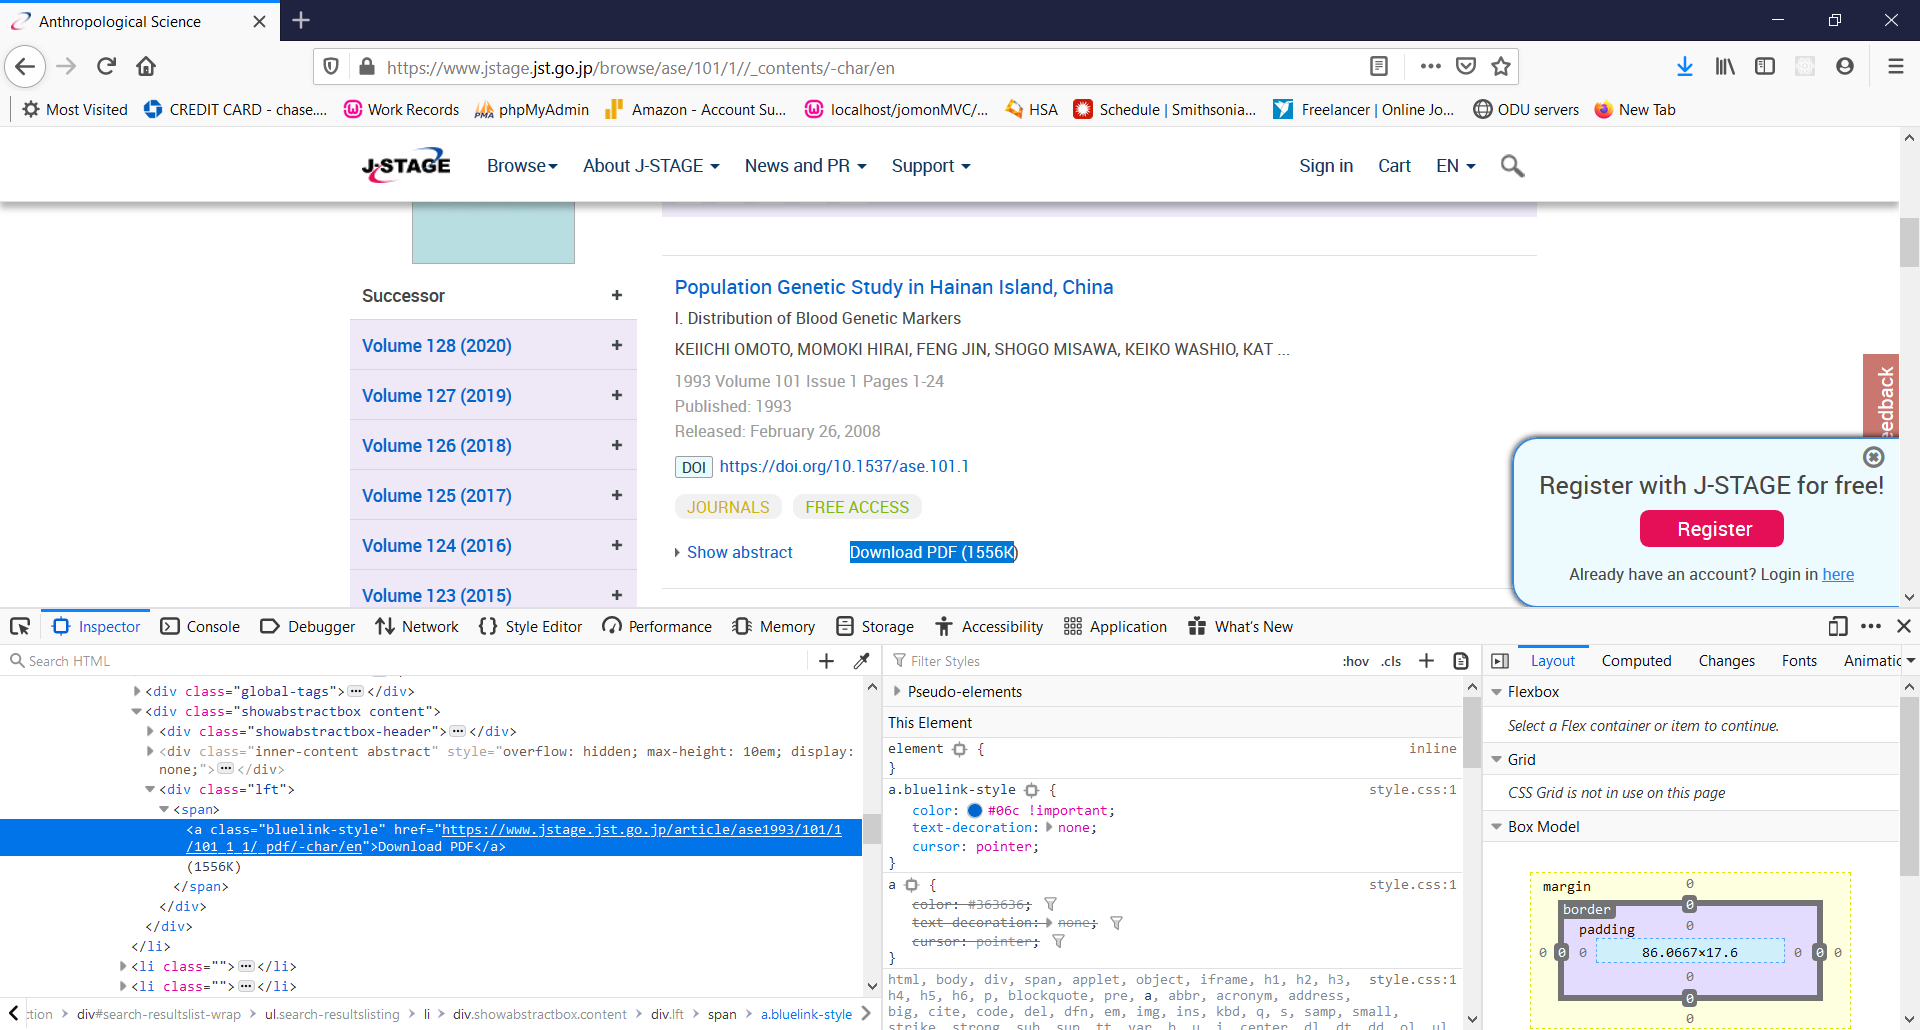
\includegraphics[trim=0 60 10 20, clip, width=\textwidth] {Q3/jstage_missingExtension.png}
    \caption{PDF links that do not end in .pdf on the JSTAGE database}
    \label{fig:q3JSTAGE_pdfs}
\end{figure}

\begin{figure}[H]
    \centering
    % trim and clip are used to crop the image, trim=left bottom right top
    % width sets max width, height will be scaled appropriately
    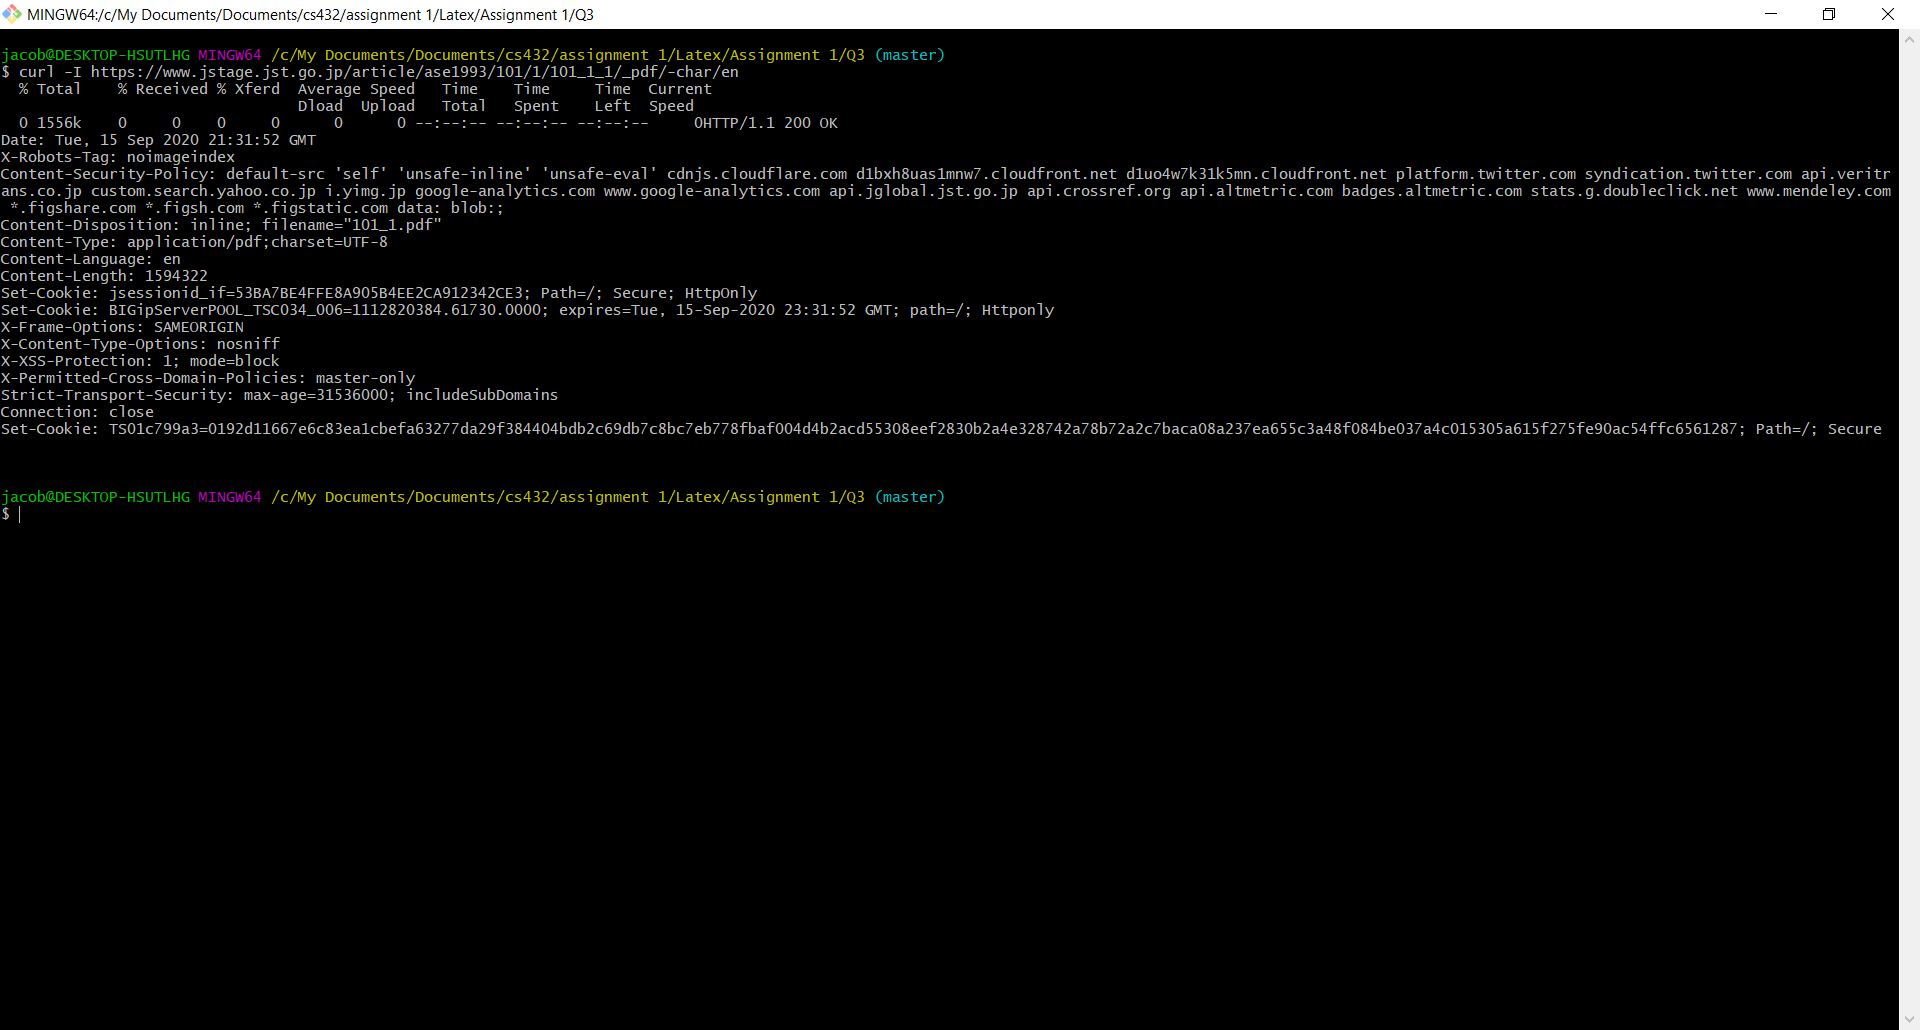
\includegraphics[trim=0 60 10 20, clip, width=\textwidth] {Q3/q3_jstage_curl.PNG}
    \caption{Headers for a pdf on JSTAGE with filename stored in content-disposition property }
    \label{fig:q3JSTAGE_headers}
\end{figure}

%referred to https://tex.stackexchange.com/questions/334899/space-between-words-in-bibliography for pacing
% referred to https://www.overleaf.com/learn/latex/bibliography_management_with_bibtex for bibtext
\RaggedRight
\bibliographystyle{elsarticle-num} 
%\bibliographystyle{unsrt}
\bibliography{references}


\end{document}

